%----------------------------------------------------------------------------------------
%	SECTION 1.5
%----------------------------------------------------------------------------------------

\section{Continuous Functions.}

\begin{definition}
    Let $X$ and  $Y$ be topological spaces. We say that a mapping $f:X
    \rightarrow Y$ is  \textbf{continuous} if for each open set $V$ in  $Y$,
    $f^{-1}(V)$ is open in $X$.
\end{definition}

Now if $f:X \rightarrow Y$ is continuous, the for every open set  $V$ of  $Y$,
$f^{-1}(V)$ is open in  $X$. Now suppose that  $\Bc$ is a basis of  $Y$, then
$V=\bingcup{B_{\alpha}}$, hence $f^{-1}(\bingcup{B_{\alpha}})$, is open in $X$

Similarly, if $\Sc$ is a subbasis of  $Y$, then for any basis element  $B$ of
$Y$,  $B=\bigcap_{i=1}^{n}{S_i}$, which then implies that
$f^{-1}(B)=\bigcap_{i=1}^{n}{f^{-1}(S_i)}$, thus $f^{-1}(S_i)$ is also open in
$X$ for $1 \leq i \leq n$.

\begin{example}
    \begin{enumerate}
        \item[(1)] Let $f:\R \rightarrow \R$ be a continuous realvalued function.
            Then for each open interval  $I \subseteq \R$,  $f^{-1}(I)$ is an
            open interval in  $\R$, so take  $x_0 \in \R$ and $\epsilon>0$, and
            let $I=(f(x_0)-\epsilon,f(x_0)+\epsilon)$, then since $ x_0 \in
            f^{-1}(I)$, there is a basis $(a,b) \subseteq f^{-1}(I)$ about
            $x_0$. Then take  $\delta=\min\{x_0-a,x_0-b\}$, then $x \in (a,b)$
            whenever $0<|x-x_0|<\delta$, and we get that $f(x) \in I$, that is,
            $|f(x)-f(x_0)|<\epsilon$. This is the definition of continuity
            defined in the real analysis. We can prove that the converse holds
            also.

            If $f:\R \rightarrow \R$ is continuous at a point $x_0$, then for
            every $\epsilon>0$, there is a  $\delta>0$ such that
            $|f(x)-f(x_0)|<\epsilon$ whenever $0<|x-x_0|<\delta$. Then we notice
            that $x$ and  $ x_0$ are distinct, furthermore, $x_0-\delta<x
            <x_0+\delta$, hence $x \in (x_0-\delta,x_0+\delta)$ implies that
            $f(x) \in (f(x_0)-\epsilon,f(x_0)+\epsilon)$. Letting
            $V_{\delta}(x_0)=(x_0-\delta,x_0+\delta) $ and
            $V_{\epsilon}(f(x_0))=(f(x_0)-\epsilon,f(x_0)+\epsilon)$, we have
            that whenever  $x \in V_{\delta}(x_0)$, then $f(x) \in
            V_{\epsilon}(f(x_0)) \subseteq f^{-1}(V_{\delta}(x_0))$. And so the
            topological definition of continuity is equivialent to the real
            analytic definition of continuity.

        \item[(2)] Let $f:\R \rightarrow \R_l$ be defined such that  $f(x)=x$ for all
            $x \in \R$. Take  $[a,b) \subseteq \R_l$, we have that
            $f^{-1}([a,b))=[a,b)$, which is not open in  $\R$  (under the
            standard topology), hence $f$ is not continuous. However, the map
            $g:\R_l \rightarrow \R$ defined the same way is continuous since
            $g^{-1}((a,b))$ is open in  $\R_l$.

        \item[(3)] Consider the map $f:\R \rightarrow \R$ defined by $f(x)=x$ if
            $x \in \Q$ and  $f(x)=0$ if $x \in \com{\R}{\Q}$. Then $f$ is
            continuous only at  $x=0$, for the limits
            \begin{equation*}
                \lim_{x \rightarrow x_0^+}{f(x)}
            \end{equation*}
            and
            \begin{equation*}
                \lim_{x \rightarrow x_0^-}{f(x)}
            \end{equation*}
            both fail to exist for $x_0 \in \Q$ and $x_0 \neq 0$.

        \item[(4)] Let $f:A \rightarrow B$ and $g:C \rightarrow D$ be continuous
            and define $f \times g:A \times C \rightarrow B \times D$ by $f
            \times g:a \times c \rightarrow f(a) \times g(c)$. Then $f \times g$
            is continous. We have that  $U$ and  $V$ open in $B$ and $D$ make
            $\inv{f}(U)$ and $\inv{g}(V)$ open in $A$ and  $C$, respectively.
            Then it follows that  $U \times V$ is open in  $B \times D$, and
            that  $\inv{(f \times g)}(U \times V)=\inv{f}(U) \times \inv{g}(V)$
            is also open by the definition if $f \times g$. This makes
            $f \times g$ continuous.
    \end{enumerate}
\end{example}

\begin{theorem}\label{1.7.1}
    Let $X$ and  $Y$ be topological spaces, and let  $f:X \rightarrow Y$ be a mapping of  $X$ into
    $Y$. Then the following are equivalent:
        \begin{enumerate}
            \item[(1)] $f$ is continuous.

            \item[(2)] For every $A \subseteq X$,  $f(\cl{A}) \subseteq \cl{f(A)}$.

            \item[(3)] For every closed set $B \subseteq Y$,  $f^{-1}(B)$ is closed in $X$.

            \item[(4)] For each  $x \in X$ and each neighborhood  $V$ of
                $f(x)$, there is a neighborhood $U$ of  $x$ such that
                $f(U) \subseteq V$.
        \end{enumerate}
\end{theorem}
\begin{proof}
    Let $f$ be continuous and let  $A \subseteq X$. Consider the neighborhood  $V$ of  $f(x)$, then
    $f^{-1}(V)$ is open in $X$, and intersects  $A$ at a point  $y$. Then  $V \cap f(A)=f(y)$, thus
    $f(x) \in \cl{f(A)}$.

    Now let $B$ be closed in  $Y$, and let  $A=f^{-1}(B)$. Then we have that
    $f(A)=f(f^{-1}(B))
    \subseteq B$, thus $x \in \cl{A}$.

    Now let $V$ be open in $Y$, so that  $B=\com{Y}{V}$ is closed in $Y$, and
    $f^{-1}(B)=\com{f^{-1}(Y)}{f^{-1}(V)}=\com{X}{f^{-1}}(V)$ which is closed in $X$, hence
    $f^{-1}(V)$ is open in $X$.

    Now let  $x \in X$, and let  $V$ be a neighborhood of  $f(x)$. Then $U=f^{-1}(V)$ is a
    neighborhood of $x$ for which  $f(U) \subseteq V$. Finally let $V$ be open in  $Y$, and let $x
    \in f^{-1}(V)$, then $f(x) \in V$, so  there is a neighborhood $U_x$ of  $x$ for which  $f(U_x) \subseteq V$,
    then $U_x \subseteq f^{-1}(V)$, then $f^{-1}(V)$ is a union of open sets, and hence open in $X$.
\end{proof}

\begin{example}\label{1.20}
    Suppose $f:X \rightarrow Y$ is continuous, and that $A \subsseteq X$. Let
    $x \in A'$ be a limit point of $A$. Certainly, we have $x \in \cl{A}$ so
    then $f(x) \in f(\cl{A}) \subseteq \cl{f(A)}$. It reamins to see if $x \in
    (f(A))'$ then. Let $V$ be open in  $Y$ such that  $x \in U=\inv{f}(V)$.
    Then $U \cap (\com{A}{x}) \neq \emptyset$. So then we get $V \cap
    (\com{f(A)}{f(x)}) \subsetq V \cap f(A) \neq \emptyset$. If $z \in U \cap A$,
    then  $f(z)=f(x)$, so that $f(U \cap A)=\{f(x)\}$, which means that $x
    \notin (f(A))'$, in general. It is the case that $f(x)$ is a limit point of
    $f(A)$ whenver $f$ is  $1-1$.
\end{example}

\begin{definition}
    Let $X$ and  $Y$ be topological spaces, and  $f:X \rightarrow Y$ be a $1-1$ mapping of  $X$ onto
    $Y$. We call  $f$ a \textbf{homeomorphism} if both $f$ and  $f^{-1}$ are continuous.
\end{definition}

\begin{lemma}\label{1.7.2}
    Let $X$ and  $Y$ be topological spaces and let $f:X \rightarrow Y$ be a homeomorphism. Then
    $f(U)$ is open if and only if $U$ is open.
\end{lemma}
\begin{proof}
    We have that both $f:X \rightarrow Y$ and  $f^{-1}:Y \rightarrow X$ are continuous $1-1$ of $X$
    and  $Y$ onto each other  (respectively). Now let $U$ be open in  $X$, then $U=f^{-1}(V)$, for
    some set  $V$ open in $Y$. Notice then, that $f(U)=f(f^{-1}(V))=V$, thus $f(U)$ is open in $Y$.
    Conversely, let $V=f(U)$ be open in $Y$ for some open set  $U$ in  $X$, then  $U=f^{-1}(V)$, so
    by definition of continuity, $U$  is open in $X$.
\end{proof}

We can also characterize now when the topology of one set is finer or coarser
than the topology of another given another given a continuous mapping.

\begin{lemma}\label{1.7.3}
    If $X$ and  $X'$ are two sets with topologies  $\Tc$ and  $\Tc'$,
    respectively,then if  $f:X' \rightarrow Y$ is the identity mapping, then $f$
    is continuous if, and only if $\Tc \subseteq \Tc'$
\end{lemma}
\begin{proof}
    Suppose that $f$ is continuous, then for every  $V$ open in  $X$ under
    $\Tc$,  $\inv{f}(V)$ is open in $X'$ unde r $\Tc'$. Since  $f$ is the
    identity, we get that $V=\inv{f}(V)$, so that $V$ is open in  $X'$.

    COnversely, if  $\Tc \subseteq \Tc'$, then for every  $V$ open in  $X$,  $V$
    is open in  $X'$. Notice then  $V=\inv{f}(V) \subseteq X'$. Therefore, $f$
    is continuous.
\end{proof}
\begin{corollary}
    $f:X' \rightarrow X$ is a homomorphism if, and only if $\Tc=\Tc'$.
\end{corollary}

\begin{definition}
    Let $X$ and  $Y$ be topological spaces and let  $f:X \rightarrow Y$ be a
    contniuous  $1-1$ maping
    of  $X$ into  $Y$, and consider  $f(X)$ as a subspace of $Y$. We call  $f:X \rightarrow f(X)$ a
    \textbf{topological imbedding} if $f$ is a homeomorphism of $X$ onto  $f(X)$.
\end{definition}

\begin{example}
    \begin{enumerate}
        \item[(1)] The map $f:\R \rightarrow \R$ defined by  $f(x)=3x+1$ is a
            homeomorphism whose inverse is $f^{-1}(y)-\frac{1}{3}(y-3)$, both
            $f$ and  $f^{-1}$ are contiuous.

        \item[(2)] The map $f:(-1,1) \rightarrow \R$ defined by $f(x)=
            \frac{x^2}{1-x^2}$ has as its inverse the map $f:\R \rightarrow
            (-1,1)$ defined by $f^{-1}(y)=\frac{2y}{1+\sqrt{1+4y^2}}$. Both $f$
            and  $f^{-1}$ are contiuous, so $f$ is a homeomorphism.

        \item[(3)] The map  $g:\R_l \rightarrow \R$ defined by  $g(x)=x$ is not
            a homeomorphism, despite being contiuous, as $g^{-1}(1)$ is undefined.

        \item[(4)] Let $S^1$ be the unit circle in $\R$, which is a subspace
            of $\R$, and define $f:[0,1) \rightarrow S^1$ by
            $f(t)=(\cos(t),\sin(t))$. Clearly $f$ is  $1-1$ onto $S^1$, and
            contiuous, however  $f^{-1}$ is not contiuous as $f([0,\frac{1}{4}))$
            is not open in $S^1$ as  $f(0)$ is in no open set of $\R^2$ such
            that  $U \cap S^1=f([0,1))$.

        \item[(5)] Consider the mappings $g:[0,1) \rightarrow \R^2$ by
            $f(t)=(\cos(2t\pi),\sin(2t\pi)))$. Now $g$ is  $1-1$ and continuous,
            and we have that  $g([0,1)) \subseteq S^1$, however since $g$ is not
            a homeomorphism,  $g$ fails to be a topological embedding.

        \item[(6)] Let $X$ and  $Y$ be topological spaces, and consider the maps
             $f:x \rightarrow x \times y_0$ and $g:y \rightarrow y_0 \times x$
             for some $x_0 \in X$ and $y_0 \in Y$. We see that $f$ and  $g$ are
             both onto $f(X)$ and $g(Y)$, respectively, and that $x \times
             y_0=x' \times y_0$ and $x_0 \times y=x_0 \times y'$ both imply that
             $x=x'$ and  $y=y'$, so  $f$ and  $g$ are also  $1-1$.

             Lastly, we see that if  $U \times y_0$ and $ x_0 \times V$ are open
             in $X \times Y$, then $\inv{f}(U \times y_0)$ and $\inv{g}(x_0
             \times V)$ are open in $X$ and  $Y$, respectively. This makes  $f$
             and  $g$ continuous, and by the same argument, so are  $\inv{f}$
             and $\inv{g}$. Thus $f$ and  $g$ are imbeddings of  $X$ onto $f(X)=
             X \times y_0$ and $g(X)=x_0 \times Y$.
    \end{enumerate}
\end{example}

\begin{theorem}[Constructions for continuous functions.]\label{1.7.4}
    Let $X$ and  $Y$ be topological spaces, then:
        \begin{enumerate}
            \item[(1)] (Constant construction) If $f:X \rightarrow Y$ maps  $x \rightarrow y_0$ for all
                $x \in X$, then  $f$ is continuous.

            \item[(2)]  (Inclusion) If $A \subseteq X$ is a subspace, then the inclusion mapping  $\iota:A
                \rightarrow Y$ is continuous.

            \item[(3)] (Construction by composition) If $f:X \rightarrow Y$ and  $g:Y \rightarrow Z$ are
                continuous, then  $f \circ g: X \rightarrow Z$ is also continuous.

            \item[(4)]  (Domain restriction) If  $f:X \rightarrow Y$ is continuous and  $A \subseteq X$,
                then  $f:A \rightarrow Y$ is continuous.

            \item[(5)]  (Range restriction) if $f:X \rightarrow Y$, and  $Z \subseteq Y$ such that  $f(X)
                \subseteq Y$, then $f:X \rightarrow Z$ is continuous.

            \item[(6)]  (Range exapnsion) If $f:X \rightarrow Y$ is continuous, and  $Y \subseteq Z$ is a
                subspace of  $Z$, then  $f:X \rightarrow Z$ is continuous.

            \item[(7)]  (Local Formulation) The map $f:X \rightarrow Y$ is continuous if  $X$ can be
                written as the union of open sets  $U_{\alpha}$ such that $f:U_{\alpha} \rightarrow
                Y$ is continuous for all $\alpha$.
        \end{enumerate}
\end{theorem}
\begin{proof}
    \begin{enumerate}
        \item[(1)] Let $f (x)=y_0$ for all $x \in X$, and let  $V$ be open in  $Y$, then  $f^{-1}(V)=X$
            or $\emptyset$ depending on if $ y_0 \in V$ or noy. In either case, $f^{-1}(V)$ is open.

        \item[(2)] If $U$ us open in  $X$, then  $f^{-1}(U)=U \cap A$ which is open in the subspace
            topology of $X$.

        \item[(3)] If $U$ is open in  $Z$,  $g^{-1}(U)$ is open in $Y$, hence  $f^{-1}g^{-1}(U)$ is
            open in $X$.

        \item[(4)] Notice that  $f_A=\iota \circ f=f:A \rightarrow Y$ which is continuous by $(2)$
            and $(3)$.

        \item[(5)] Let $f:A \rightarrow Y$ be continuous and let  $f(X) \subseteq Z \subseteq Y$. Let $B$
            be open in  $Z$, so  $B=Z \cap U$ for some  $U$ open in  $Y$. Now by hypothesis, we have
            that $f^{-1}(U) \subseteq f^{-1}(B)$, hence $f^{-1}(B)$ is open in $X$, thus  $f:X
            \rightarrow Z$ is continuous.

        \item[(6)] Let  $f$ be as in  $(5)$, and let $Y \subseteq Z$ be a subspace of  $Z$. Then the
            mapping  $h:X \rightarrow Z$ defined by $h=\iota \circ f$ is continuous.

        \item[(7)] Let  $X=\bingcup{U_{\alpha}}$ where $U_{\alpha}$ is open in $X$, and $f:U_{\alpha}
            \rightarrow Y$ is continuous for all  $\alpha$. Let $V$ be open in  $Y$, then
            $f^{-1}(V) \cap U_{\alpha}=f^{-1}_U{\alpha}(V)$, and since $f$ is continuous on
            $U_{\alpha}$, then $f^{-1}(V)=\bigcup{f^{-1}_{U_{\alpha}}(V)}$ is open in $X$.
    \end{enumerate}
\end{proof}

\begin{theorem}[The pasting lemma]\label{1.7.5}
    Let $X=A \cup B$ with  $A$ and  $B$ closed in  $X$, and let  $f:A \rightarrow Y$ and  $g:B
    \rightarrow Y$ be continuous. If  $f(x)=g(x)$ for all $x \in A \cap B$, then we can
    construct a mapping  $h:X \rightarrow Y$ defined by  $h(x)=
        \begin{cases}
            f(x) \text{, } & x \in A \\
            g(x) \text{, } & x \in B
        \end{cases}$
    . Then $h$ is continuous.
\end{theorem}
\begin{proof}
    Let $C$ be closed in  $Y$, then  $h^{-1}(C)=f^{-1}(C) \cup g^{-1}(C)$. Since $f$ and  $g$ are
    continuous, then  $f^{-1}(C)$ and $g^{-1}(C)$ are closed in $A$ and  $B$, respectively. Thus
    $h^{-1}(C)$ is closed in $X$.
\end{proof}

\begin{example}
        Define $h:\R \rightarrow \R$ by $h(x)=
            \begin{cases}
                x \text{, } & x \leq 0 \\
                \frac{x}{2} \text{, } & x \geq 0
            \end{cases}$
        . We have that $x$ and  $\frac{x}{2}$ are continuous on their respective domains,
        intersecting at $0$, i.e.  $x:(-\infty,0] \rightarrow \R$, $ \frac{x}{2}:[0,\infty
        \rightarrow \R$, and $\{0\}=(-\infty, 0] \cap [0, \infty)$. Thus $h$ is continuous on $\R$.


        However, $k,l:\R \rightarrow \R$ defined by $k(x)=
            \begin{cases}
                x-2 \text{, } & x \leq 0 \\
                x+2 \text{, } & x \geq 0
            \end{cases}$
            and $l(x)=
            \begin{cases}
                x-2 \text{, } & x < 0 \\
                x+2 \text{, } & x \geq 0
            \end{cases}$
            are not continuous. We have that their domains intersect at $0$, but that  $k(0)=\pm_2$,
            (so $k$ isn't even a function). Likewise, $(-\infty,0) \cap [0,\infty)=\emptyset$, which
            is open in $\R$ see \ref{fig_1.9}.

            \begin{figure}[h]
                \centering
                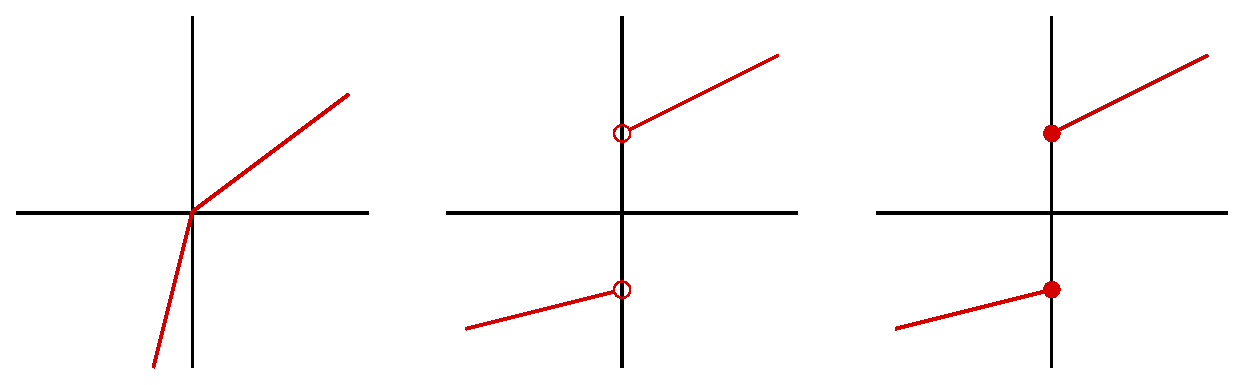
\includegraphics[scale = 0.5]{Figures/Chapter1/pasting_lemma.eps}
                \caption{The mappings $h$, $k$, and  $l$.}
                \label{fig_1.9}
            \end{figure}
\end{example}

\begin{theorem}\label{1.7.5}
    Let $f:A \rightarrow X \times Y$ be defined by  $f(a)=(f_1(a),f_2(a))$, where $ f_1:A
    \rightarrow X$ and $ f_2: A \rightarrow Y$. Then $f$ is continuous if and only if  $ f_1$ and $
    f_2$ are continuous.
\end{theorem}
\begin{proof}
    Let $\pi_1:X \times Y \rightarrow X$ and $\pi_2:X \times Y \rightarrow Y$ be projections onto
    $X$ and  $Y$ respectively. Since  $\pi_1^{-1}(U)=U \times Y$ and $\pi_2^{-1}(V)=X \times V$ are
    both open in  $X \times Y$,  $\pi_1$ and $\pi_2$ are continuous. Then notice that $ f_1(a)=\pi_1
    \circ f(a)$ and $ f_2(a)=\pi_2 \circ f(a)$, both of which are continuous.

    Now suppose that $ f_1$ and $ f_2$ are continuous..We have that $a \in f^{-1}(U \times V)$ if
    and only if $f_1(a) \in U$ and $ f_2(a) \in V$, then $ f_1^{-1}(U)$ and $f_2^{-1}(V)$ are open
    in $A$, hence so is $f^{-1}(U \times V)=f_1^{-1}(U) \cap f_2^{-1}(V)$.
\end{proof}

We now conclude the section with some more definitions and examples.

\begin{definition}
    We define the \textbf{parametrized curve} of the plane $\R^2$ to be the continuous function
    $f:[a,b] \rightarrow \R^2$ defined by $f(t)=(x(t),y(t))$. If $f$ is in a vector field, then wwe
    define $f(t)=x(t)i+y(t)j$ where $i=
    \begin{pmatrix}
        1 \\
        0
    \end{pmatrix}$
    and $j=
    \begin{pmatrix}
        0 \\
        1
    \end{pmatrix}$
\end{definition}

\begin{example}
    The function $f(t)=((\cos(t)),\sin(t))$ is a parametrization of the curve $x^2+y^2=1$, i.e. the
    unit circle  $S^1$.
\end{example}

\begin{example}\label{1.24}
    Suppose $\{A_\alpha\}$ is a finite collection of subsets of a topological
    space $X$, and that  $X=\bigcup_{\alpha}{A_\alpha}$. Suppose $f:X
    \rightarrow Y$ is defined such that the maps $f_\alpha=f:A_\alpha
    \rightarrow Y$ are continuous for each $\alpha$. Then  $f$ is also
    continuous provided that each  $A_\alpha$ is closed. For, if each
    $A_\alpha$ is closed, then  $X$ is the finite union of closed sets.
    Morevoer, for any  $V \subseteq Y$ closed, we get  $\inv{f_\alpha}(V)$ is
    closed in $A_\alpha$ as a subspace of  $X$. So
    $\inv{f}(V)=\bigcup{\inv{f_\alpha}(V)}$ is closed in $X=\bigcup{A_\alpha}$,
    via local formulation, Making $f$ continuous.

    This fact is not true however if  $\{A_\alpha\}$ is countable, but not
    finite. Consider the collection $\{[\frac{1}{n},1]\}_{n \in \Z^+}$, of the
    space $[0,1]$. We have $[0,1]=\bigcup_{n \in \Z^+}{[\frac{1}{n}, 1]}$, and
    each $[\frac{1}{n},1]$ is closed in $[0,1]$ as a subspace of $\R$. However,
    the function  $f(x)=\frac{1}{n}$ if $x \in [\frac{1}{n}, 1]$ and $f(x)=1$
    otherwise is continuous on each $[\frac{1}{n},1]$, but its local formulation
    is not continuous on $[0,1]$.
\end{example}

\begin{remark}
    Theorem \ref{1.7.4} only states that the local formulation of a mapping is
    continuous only if its domain is the union of open sets. Thus a local
    formulation where the domain is a union of closed sets need not be
    continuous.
\end{remark}

\begin{definition}
    Let $X$ be a topological space, and  $\{A_\alpha\}$ a collection of subsets
    of $X$. We call \$ {a_\alpha\} \textbf{locally finite} if for each $x \in
    X$, there is a neighborhood  $U$ of  $X$ such that  $U \cap A_\alpha \neq
    \emptyset$ only for a finite number of  $\alpha$.
\end{definition}

\begin{lemma}\label{1.7.7}
    Let $X$ be a topological space, and  $\{A_\alpha\}$ a locally finite
    collection of subsets of $X$. If  $f:X \rightarrow Y$ is defined such that
    $f_\alpha=f:A_\alpha \rightarrow Y$ is continuous for each $\alpha$, then
    $f$ is continuou.
\end{lemma}
\begin{proof}
    If $\{A_\alpha\}$ is locally finite, then for each $x \in X$, there s a
    neighborhood  $U_x$ of  $x$ such that  $U_x \cap A_\alpha \neq \emptyset$
    for only a finite number of  $\alpha$. Then  $U_x \cap A_\alpha$ is open in
     $A_\alpha$ as a subspace of  $X$. Then  $V_x=\com{A_\alpha}{(U_x \cap
     A_\alpha)}$ is closed in $A_\alpha$, and  $V_x=\inv{f_\alpha}(W)$ for some
     $W$ closed in  $Y$. Thus  $\bigcup_{x \in
     X}{V_x}=\bigcup_{\alpha}{\inv{f_\alpha}(W)}=\inv{f}(W)$ (which is a finite
     union) is closed in $X$. This makes $f$ continuous.
\end{proof}

\begin{definition}
    Let $X$,  $Y$, and  $Z$ be topological space. We say a map  $F: X \times Y
    \rightarrow Z$ is \textbf{continuous in each variable} if the maps $F_X:X
    \rightarrow Z$ and $F_Y:Y \rightarrow Z$ defined by $F_X(x)=F(x \times y_0)$
    and $F_Y(y)=F(x_0 \times y)$ are continuous.
\end{definition}

\begin{lemma}\label{1.7.8}
    If $X$,  $Y$, and  $Z$ are topological spaces, and  $F:X \times Y
    \rightarrow Z$ is continuous, then $F$ is continuous in each variable
    seperately.
\end{lemma}
\begin{proof}
    If $F$ is continuous, then  $W$ open in  $Z$ implies that $\inv{F}(W)$ is
    open in $X \times Y$, and that  $U \times V=\inv{F}(W)$ for $U$ and  $V$
    open in  $X$ and  $Y$ respectively. Then $F$ is continuous at $U \times
    y_0$, for $y_0 \in V$; that is $\inv{F}(U \times y_0)$ is open in $X \times
    Y$. So, by definition,  $F_X(U)$ is open in $X$, and $F_X$ is continuous.
    By similar reasoning, we can also conclude that $F_Y$ is continuous, and
    that $F$ is continuous in each variable.
\end{proof}

\begin{example}\label{1.25}
    Define $F:\R \rightarrow \R$ by
    \begin{equation*}
        F(x \times y)=\begin{cases}
                    \frac{xy}{x^2+y^2}, \text{ if } x \times y \neq 0 \times 0 \\
                    0, \text{ otherwise}
                \end{cases}
    \end{equation*}
    Define $F_X(x)=F(x \times y_0)$, then $F(x \times
    y_0)=\frac{xy_0}{x^2+y_0^2}$ if $x \neq 0$ and  $y_0 \neq 0$, and $0$
    otherwise. Then when $y_0=0$ we see that
    \begin{equation*}
        \lim_{x \rightarrow 0}{F(x \times y_0)}=\lim_{x \rightarrow 0}{F_X(x)}
        =F_X(0)=F(0 \times 0)=0
    \end{equation*}
    so that $F_X$ is continuous at  $x=0$, and it is also continuous everywhere
    else. So  $F_X$ is continuous. Similarly, the mapping  $F_Y(y)=F(x_0 \times
    y)$ is also continuous, and $F$ is continous in each variable.

     $F$ however, is not continuous in general. Define  $g(x)=F(x \times x)$ so
     we get
     \begin{equation*}
         g(x)=\begin{cases}
                \frac{1}{2}, \text{ if } x \neq 0 \\
                0, \text{ otherwise}
            \end{cases}
     \end{equation*}
     which is not continuous. So $F$ cannot be continuous at the points  $x
     \times x$, for it degenrates into a noncontinuous function. In fact, if we
     have $\frac{xy}{x^2+y^2}=\frac{1}{2}$, then we get $x^2+y^2-2xy=(x-y)^2=0$
     and $x \times y \neq 0 \times 0$. This means $\inv{F}(\{\frac{1}{2}\})=\{x
     \times x : x \neq 0\}$ is not closed.
\end{example}
